\documentclass[12pt,a4paper]{article}

\usepackage{import}
\usepackage{amssymb}
\import{../../00Notes_and_Summaries/Template/}{format.tex}

\newcommand{\topic}{Statistics coursework}

\begin{document}

\title{\topic}
\begin{titlepage}
    \maketitle
\end{titlepage}

\tableofcontents

\newpage
\begin{abstract}
\noindent
\end{abstract}

\section{Introduction}
\section{Geometric relationship}
This section corresponds to the question \textbf{i}. I am going to compute the geometric relationship between $\alpha$, $\beta$, $\theta$ and $x$.
$alpha$ and $\beta$ are the coordinates of the lighthouse on the map. i.e. the lighthouse is at position $alpha$ along a straight coastline and a distance $\beta$  out to sea. 

Given that the angle which the light emits are uniformly distributed between $-\pi/2$ and $\pi/2$, we can write the probability density function of the angle as:
\begin{equation}
    f(\theta) = \frac{1}{\pi} \quad \text{for} \quad -\frac{\pi}{2} \leq \theta \leq \frac{\pi}{2}
\end{equation}
The geometric relationship between $\alpha$, $\beta$, $\theta$ and $x$ is shown in the figure \ref{fig:geometry}.
$$
    \tan\theta = \frac{\alpha-x}{\beta}
$$
from which we derive the infinitesimal relationship between $\theta$ and $x$ as:
\begin{equation}
    {dx} = \beta \sec^2\theta d\theta
\end{equation}
We know the relationship between $\theta$ and $x$ is given by:
\begin{equation}
    p_{\theta}(\theta) d\theta = p_{x}(x) dx
\end{equation}
Therefore
\begin{align*}
    p_{x}(x) &= p_{\theta}(\theta) \frac{d\theta}{dx} \\
    &= \frac{1}{\pi} \frac{1}{\beta\sec^2\theta} \\
    &= \frac{1}{\pi\beta} \cos^2\theta\\
    &= \frac{1}{\pi\beta} \frac{\beta^2}{\beta^2 + (x-\alpha)^2}\\
    &= \frac{\beta}{\pi(\beta^2 + (x-\alpha)^2)}
\end{align*}
\begin{figure}[H]
    \centering
    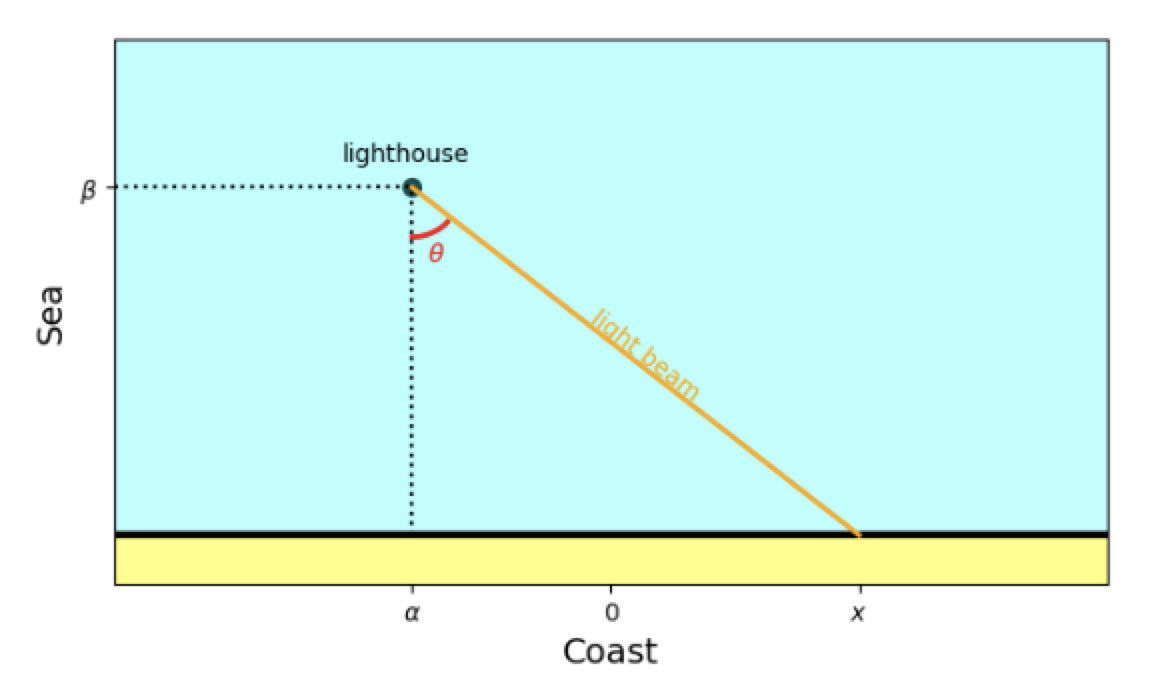
\includegraphics[width=0.5\textwidth]{figures/lighthouse.png}
    \caption{Geometric relationship between $\alpha$, $\beta$, $\theta$ and $x$}
    \label{fig:geometry}
\end{figure}
\section{Best estimator for $\alpha$}
This section corresponds to the question \textbf{iii}.
First, it could be shown that the 
\end{document}